


% Header, overrides base

    % Make sure that the sphinx doc style knows who it inherits from.
    \def\sphinxdocclass{article}

    % Declare the document class
    \documentclass[letterpaper,10pt,english]{/Library/Python/2.7/site-packages/sphinx/texinputs/sphinxhowto}

    % Imports
    \usepackage[utf8]{inputenc}
    \DeclareUnicodeCharacter{00A0}{\\nobreakspace}
    \usepackage[T1]{fontenc}
    \usepackage{babel}
    \usepackage{times}
    \usepackage{import}
    \usepackage[Bjarne]{/Library/Python/2.7/site-packages/sphinx/texinputs/fncychap}
    \usepackage{longtable}
    \usepackage{/Library/Python/2.7/site-packages/sphinx/texinputs/sphinx}
    \usepackage{multirow}

    \usepackage{amsmath}
    \usepackage{amssymb}
    \usepackage{ucs}
    \usepackage{enumerate}

    % Used to make the Input/Output rules follow around the contents.
    \usepackage{needspace}

    % Pygments requirements
    \usepackage{fancyvrb}
    \usepackage{color}
    % ansi colors additions
    \definecolor{darkgreen}{rgb}{.12,.54,.11}
    \definecolor{lightgray}{gray}{.95}
    \definecolor{brown}{rgb}{0.54,0.27,0.07}
    \definecolor{purple}{rgb}{0.5,0.0,0.5}
    \definecolor{darkgray}{gray}{0.25}
    \definecolor{lightred}{rgb}{1.0,0.39,0.28}
    \definecolor{lightgreen}{rgb}{0.48,0.99,0.0}
    \definecolor{lightblue}{rgb}{0.53,0.81,0.92}
    \definecolor{lightpurple}{rgb}{0.87,0.63,0.87}
    \definecolor{lightcyan}{rgb}{0.5,1.0,0.83}

    % Needed to box output/input
    \usepackage{tikz}
        \usetikzlibrary{calc,arrows,shadows}
    \usepackage[framemethod=tikz]{mdframed}

    \usepackage{alltt}

    % Used to load and display graphics
    \usepackage{graphicx}
    \graphicspath{ {figs/} }
    \usepackage[Export]{adjustbox} % To resize

    % used so that images for notebooks which have spaces in the name can still be included
    \usepackage{grffile}


    % For formatting output while also word wrapping.
    \usepackage{listings}
    \lstset{breaklines=true}
    \lstset{basicstyle=\small\ttfamily}
    \def\smaller{\fontsize{9.5pt}{9.5pt}\selectfont}

    %Pygments definitions
    
\makeatletter
\def\PY@reset{\let\PY@it=\relax \let\PY@bf=\relax%
    \let\PY@ul=\relax \let\PY@tc=\relax%
    \let\PY@bc=\relax \let\PY@ff=\relax}
\def\PY@tok#1{\csname PY@tok@#1\endcsname}
\def\PY@toks#1+{\ifx\relax#1\empty\else%
    \PY@tok{#1}\expandafter\PY@toks\fi}
\def\PY@do#1{\PY@bc{\PY@tc{\PY@ul{%
    \PY@it{\PY@bf{\PY@ff{#1}}}}}}}
\def\PY#1#2{\PY@reset\PY@toks#1+\relax+\PY@do{#2}}

\expandafter\def\csname PY@tok@gd\endcsname{\def\PY@tc##1{\textcolor[rgb]{0.63,0.00,0.00}{##1}}}
\expandafter\def\csname PY@tok@gu\endcsname{\let\PY@bf=\textbf\def\PY@tc##1{\textcolor[rgb]{0.50,0.00,0.50}{##1}}}
\expandafter\def\csname PY@tok@gt\endcsname{\def\PY@tc##1{\textcolor[rgb]{0.00,0.25,0.82}{##1}}}
\expandafter\def\csname PY@tok@gs\endcsname{\let\PY@bf=\textbf}
\expandafter\def\csname PY@tok@gr\endcsname{\def\PY@tc##1{\textcolor[rgb]{1.00,0.00,0.00}{##1}}}
\expandafter\def\csname PY@tok@cm\endcsname{\let\PY@it=\textit\def\PY@tc##1{\textcolor[rgb]{0.25,0.50,0.50}{##1}}}
\expandafter\def\csname PY@tok@vg\endcsname{\def\PY@tc##1{\textcolor[rgb]{0.10,0.09,0.49}{##1}}}
\expandafter\def\csname PY@tok@m\endcsname{\def\PY@tc##1{\textcolor[rgb]{0.40,0.40,0.40}{##1}}}
\expandafter\def\csname PY@tok@mh\endcsname{\def\PY@tc##1{\textcolor[rgb]{0.40,0.40,0.40}{##1}}}
\expandafter\def\csname PY@tok@go\endcsname{\def\PY@tc##1{\textcolor[rgb]{0.50,0.50,0.50}{##1}}}
\expandafter\def\csname PY@tok@ge\endcsname{\let\PY@it=\textit}
\expandafter\def\csname PY@tok@vc\endcsname{\def\PY@tc##1{\textcolor[rgb]{0.10,0.09,0.49}{##1}}}
\expandafter\def\csname PY@tok@il\endcsname{\def\PY@tc##1{\textcolor[rgb]{0.40,0.40,0.40}{##1}}}
\expandafter\def\csname PY@tok@cs\endcsname{\let\PY@it=\textit\def\PY@tc##1{\textcolor[rgb]{0.25,0.50,0.50}{##1}}}
\expandafter\def\csname PY@tok@cp\endcsname{\def\PY@tc##1{\textcolor[rgb]{0.74,0.48,0.00}{##1}}}
\expandafter\def\csname PY@tok@gi\endcsname{\def\PY@tc##1{\textcolor[rgb]{0.00,0.63,0.00}{##1}}}
\expandafter\def\csname PY@tok@gh\endcsname{\let\PY@bf=\textbf\def\PY@tc##1{\textcolor[rgb]{0.00,0.00,0.50}{##1}}}
\expandafter\def\csname PY@tok@ni\endcsname{\let\PY@bf=\textbf\def\PY@tc##1{\textcolor[rgb]{0.60,0.60,0.60}{##1}}}
\expandafter\def\csname PY@tok@nl\endcsname{\def\PY@tc##1{\textcolor[rgb]{0.63,0.63,0.00}{##1}}}
\expandafter\def\csname PY@tok@nn\endcsname{\let\PY@bf=\textbf\def\PY@tc##1{\textcolor[rgb]{0.00,0.00,1.00}{##1}}}
\expandafter\def\csname PY@tok@no\endcsname{\def\PY@tc##1{\textcolor[rgb]{0.53,0.00,0.00}{##1}}}
\expandafter\def\csname PY@tok@na\endcsname{\def\PY@tc##1{\textcolor[rgb]{0.49,0.56,0.16}{##1}}}
\expandafter\def\csname PY@tok@nb\endcsname{\def\PY@tc##1{\textcolor[rgb]{0.00,0.50,0.00}{##1}}}
\expandafter\def\csname PY@tok@nc\endcsname{\let\PY@bf=\textbf\def\PY@tc##1{\textcolor[rgb]{0.00,0.00,1.00}{##1}}}
\expandafter\def\csname PY@tok@nd\endcsname{\def\PY@tc##1{\textcolor[rgb]{0.67,0.13,1.00}{##1}}}
\expandafter\def\csname PY@tok@ne\endcsname{\let\PY@bf=\textbf\def\PY@tc##1{\textcolor[rgb]{0.82,0.25,0.23}{##1}}}
\expandafter\def\csname PY@tok@nf\endcsname{\def\PY@tc##1{\textcolor[rgb]{0.00,0.00,1.00}{##1}}}
\expandafter\def\csname PY@tok@si\endcsname{\let\PY@bf=\textbf\def\PY@tc##1{\textcolor[rgb]{0.73,0.40,0.53}{##1}}}
\expandafter\def\csname PY@tok@s2\endcsname{\def\PY@tc##1{\textcolor[rgb]{0.73,0.13,0.13}{##1}}}
\expandafter\def\csname PY@tok@vi\endcsname{\def\PY@tc##1{\textcolor[rgb]{0.10,0.09,0.49}{##1}}}
\expandafter\def\csname PY@tok@nt\endcsname{\let\PY@bf=\textbf\def\PY@tc##1{\textcolor[rgb]{0.00,0.50,0.00}{##1}}}
\expandafter\def\csname PY@tok@nv\endcsname{\def\PY@tc##1{\textcolor[rgb]{0.10,0.09,0.49}{##1}}}
\expandafter\def\csname PY@tok@s1\endcsname{\def\PY@tc##1{\textcolor[rgb]{0.73,0.13,0.13}{##1}}}
\expandafter\def\csname PY@tok@sh\endcsname{\def\PY@tc##1{\textcolor[rgb]{0.73,0.13,0.13}{##1}}}
\expandafter\def\csname PY@tok@sc\endcsname{\def\PY@tc##1{\textcolor[rgb]{0.73,0.13,0.13}{##1}}}
\expandafter\def\csname PY@tok@sx\endcsname{\def\PY@tc##1{\textcolor[rgb]{0.00,0.50,0.00}{##1}}}
\expandafter\def\csname PY@tok@bp\endcsname{\def\PY@tc##1{\textcolor[rgb]{0.00,0.50,0.00}{##1}}}
\expandafter\def\csname PY@tok@c1\endcsname{\let\PY@it=\textit\def\PY@tc##1{\textcolor[rgb]{0.25,0.50,0.50}{##1}}}
\expandafter\def\csname PY@tok@kc\endcsname{\let\PY@bf=\textbf\def\PY@tc##1{\textcolor[rgb]{0.00,0.50,0.00}{##1}}}
\expandafter\def\csname PY@tok@c\endcsname{\let\PY@it=\textit\def\PY@tc##1{\textcolor[rgb]{0.25,0.50,0.50}{##1}}}
\expandafter\def\csname PY@tok@mf\endcsname{\def\PY@tc##1{\textcolor[rgb]{0.40,0.40,0.40}{##1}}}
\expandafter\def\csname PY@tok@err\endcsname{\def\PY@bc##1{\setlength{\fboxsep}{0pt}\fcolorbox[rgb]{1.00,0.00,0.00}{1,1,1}{\strut ##1}}}
\expandafter\def\csname PY@tok@kd\endcsname{\let\PY@bf=\textbf\def\PY@tc##1{\textcolor[rgb]{0.00,0.50,0.00}{##1}}}
\expandafter\def\csname PY@tok@ss\endcsname{\def\PY@tc##1{\textcolor[rgb]{0.10,0.09,0.49}{##1}}}
\expandafter\def\csname PY@tok@sr\endcsname{\def\PY@tc##1{\textcolor[rgb]{0.73,0.40,0.53}{##1}}}
\expandafter\def\csname PY@tok@mo\endcsname{\def\PY@tc##1{\textcolor[rgb]{0.40,0.40,0.40}{##1}}}
\expandafter\def\csname PY@tok@kn\endcsname{\let\PY@bf=\textbf\def\PY@tc##1{\textcolor[rgb]{0.00,0.50,0.00}{##1}}}
\expandafter\def\csname PY@tok@mi\endcsname{\def\PY@tc##1{\textcolor[rgb]{0.40,0.40,0.40}{##1}}}
\expandafter\def\csname PY@tok@gp\endcsname{\let\PY@bf=\textbf\def\PY@tc##1{\textcolor[rgb]{0.00,0.00,0.50}{##1}}}
\expandafter\def\csname PY@tok@o\endcsname{\def\PY@tc##1{\textcolor[rgb]{0.40,0.40,0.40}{##1}}}
\expandafter\def\csname PY@tok@kr\endcsname{\let\PY@bf=\textbf\def\PY@tc##1{\textcolor[rgb]{0.00,0.50,0.00}{##1}}}
\expandafter\def\csname PY@tok@s\endcsname{\def\PY@tc##1{\textcolor[rgb]{0.73,0.13,0.13}{##1}}}
\expandafter\def\csname PY@tok@kp\endcsname{\def\PY@tc##1{\textcolor[rgb]{0.00,0.50,0.00}{##1}}}
\expandafter\def\csname PY@tok@w\endcsname{\def\PY@tc##1{\textcolor[rgb]{0.73,0.73,0.73}{##1}}}
\expandafter\def\csname PY@tok@kt\endcsname{\def\PY@tc##1{\textcolor[rgb]{0.69,0.00,0.25}{##1}}}
\expandafter\def\csname PY@tok@ow\endcsname{\let\PY@bf=\textbf\def\PY@tc##1{\textcolor[rgb]{0.67,0.13,1.00}{##1}}}
\expandafter\def\csname PY@tok@sb\endcsname{\def\PY@tc##1{\textcolor[rgb]{0.73,0.13,0.13}{##1}}}
\expandafter\def\csname PY@tok@k\endcsname{\let\PY@bf=\textbf\def\PY@tc##1{\textcolor[rgb]{0.00,0.50,0.00}{##1}}}
\expandafter\def\csname PY@tok@se\endcsname{\let\PY@bf=\textbf\def\PY@tc##1{\textcolor[rgb]{0.73,0.40,0.13}{##1}}}
\expandafter\def\csname PY@tok@sd\endcsname{\let\PY@it=\textit\def\PY@tc##1{\textcolor[rgb]{0.73,0.13,0.13}{##1}}}

\def\PYZbs{\char`\\}
\def\PYZus{\char`\_}
\def\PYZob{\char`\{}
\def\PYZcb{\char`\}}
\def\PYZca{\char`\^}
\def\PYZam{\char`\&}
\def\PYZlt{\char`\<}
\def\PYZgt{\char`\>}
\def\PYZsh{\char`\#}
\def\PYZpc{\char`\%}
\def\PYZdl{\char`\$}
\def\PYZti{\char`\~}
% for compatibility with earlier versions
\def\PYZat{@}
\def\PYZlb{[}
\def\PYZrb{]}
\makeatother


    %Set pygments styles if needed...
    
        \definecolor{nbframe-border}{rgb}{0.867,0.867,0.867}
        \definecolor{nbframe-bg}{rgb}{0.969,0.969,0.969}
        \definecolor{nbframe-in-prompt}{rgb}{0.0,0.0,0.502}
        \definecolor{nbframe-out-prompt}{rgb}{0.545,0.0,0.0}

        \newenvironment{ColorVerbatim}
        {\begin{mdframed}[%
            roundcorner=1.0pt, %
            backgroundcolor=nbframe-bg, %
            userdefinedwidth=1\linewidth, %
            leftmargin=0.1\linewidth, %
            innerleftmargin=0pt, %
            innerrightmargin=0pt, %
            linecolor=nbframe-border, %
            linewidth=1pt, %
            usetwoside=false, %
            everyline=true, %
            innerlinewidth=3pt, %
            innerlinecolor=nbframe-bg, %
            middlelinewidth=1pt, %
            middlelinecolor=nbframe-bg, %
            outerlinewidth=0.5pt, %
            outerlinecolor=nbframe-border, %
            needspace=0pt
        ]}
        {\end{mdframed}}
        
        \newenvironment{InvisibleVerbatim}
        {\begin{mdframed}[leftmargin=0.1\linewidth,innerleftmargin=3pt,innerrightmargin=3pt, userdefinedwidth=1\linewidth, linewidth=0pt, linecolor=white, usetwoside=false]}
        {\end{mdframed}}

        \renewenvironment{Verbatim}[1][\unskip]
        {\begin{alltt}\smaller}
        {\end{alltt}}
    

    % Help prevent overflowing lines due to urls and other hard-to-break 
    % entities.  This doesn't catch everything...
    \sloppy

    % Document level variables
    \title{Section2\_1-IPython}
    \date{August 20, 2013}
    \release{}
    \author{Unknown Author}
    \renewcommand{\releasename}{}

    % TODO: Add option for the user to specify a logo for his/her export.
    \newcommand{\sphinxlogo}{}

    % Make the index page of the document.
    \makeindex

    % Import sphinx document type specifics.
     


% Body

    % Start of the document
    \begin{document}

        
            \maketitle
        

        


        
        \section{IPython}

\textbf{IPython} is an enhanced Python shell which provides a more
robust and productive development environment for users. There are
several key features that set it apart from the standard Python shell .

\subsubsection{History}

In IPython, all your inputs and outputs are saved. There are two
variables named \texttt{In} and \texttt{Out} which are assigned as you
work with your results. All outputs are saved automatically to variables
of the form \texttt{\_N}, where \texttt{N} is the prompt number, and
inputs to \texttt{\_iN}. This allows you to recover quickly the result
of a prior computation by referring to its number even if you forgot to
store it as a variable.

    % Make sure that atleast 4 lines are below the HR
    \needspace{4\baselineskip}

    
        \vspace{6pt}
        \makebox[0.1\linewidth]{\smaller\hfill\tt\color{nbframe-in-prompt}In\hspace{4pt}{[}{]}:\hspace{4pt}}\\*
        \vspace{-2.65\baselineskip}
        \begin{ColorVerbatim}
            \vspace{-0.7\baselineskip}
            \begin{Verbatim}[commandchars=\\\{\}]
\PY{n}{np}\PY{o}{.}\PY{n}{sin}\PY{p}{(}\PY{l+m+mi}{4}\PY{p}{)}\PY{o}{*}\PY{o}{*}\PY{l+m+mi}{2}
\end{Verbatim}

            
                \vspace{-0.2\baselineskip}
            
        \end{ColorVerbatim}
    


    % Make sure that atleast 4 lines are below the HR
    \needspace{4\baselineskip}

    
        \vspace{6pt}
        \makebox[0.1\linewidth]{\smaller\hfill\tt\color{nbframe-in-prompt}In\hspace{4pt}{[}{]}:\hspace{4pt}}\\*
        \vspace{-2.65\baselineskip}
        \begin{ColorVerbatim}
            \vspace{-0.7\baselineskip}
            \begin{Verbatim}[commandchars=\\\{\}]
\PY{n}{\PYZus{}28}
\end{Verbatim}

            
                \vspace{-0.2\baselineskip}
            
        \end{ColorVerbatim}
    


    % Make sure that atleast 4 lines are below the HR
    \needspace{4\baselineskip}

    
        \vspace{6pt}
        \makebox[0.1\linewidth]{\smaller\hfill\tt\color{nbframe-in-prompt}In\hspace{4pt}{[}{]}:\hspace{4pt}}\\*
        \vspace{-2.65\baselineskip}
        \begin{ColorVerbatim}
            \vspace{-0.7\baselineskip}
            \begin{Verbatim}[commandchars=\\\{\}]
\PY{n}{\PYZus{}i28}
\end{Verbatim}

            
                \vspace{-0.2\baselineskip}
            
        \end{ColorVerbatim}
    


    % Make sure that atleast 4 lines are below the HR
    \needspace{4\baselineskip}

    
        \vspace{6pt}
        \makebox[0.1\linewidth]{\smaller\hfill\tt\color{nbframe-in-prompt}In\hspace{4pt}{[}{]}:\hspace{4pt}}\\*
        \vspace{-2.65\baselineskip}
        \begin{ColorVerbatim}
            \vspace{-0.7\baselineskip}
            \begin{Verbatim}[commandchars=\\\{\}]
\PY{n}{\PYZus{}28} \PY{o}{/} \PY{l+m+mf}{4.}
\end{Verbatim}

            
                \vspace{-0.2\baselineskip}
            
        \end{ColorVerbatim}
    
\subsubsection{Introspection}

If you want details regarding the properties and functionality of any
Python objects currently loaded into IPython, you can use the \texttt{?}
to reveal any details that are available:

    % Make sure that atleast 4 lines are below the HR
    \needspace{4\baselineskip}

    
        \vspace{6pt}
        \makebox[0.1\linewidth]{\smaller\hfill\tt\color{nbframe-in-prompt}In\hspace{4pt}{[}{]}:\hspace{4pt}}\\*
        \vspace{-2.65\baselineskip}
        \begin{ColorVerbatim}
            \vspace{-0.7\baselineskip}
            \begin{Verbatim}[commandchars=\\\{\}]
\PY{n}{some\PYZus{}dict} \PY{o}{=} \PY{p}{\PYZob{}}\PY{p}{\PYZcb{}}
\PY{n}{some\PYZus{}dict}\PY{err}{?}
\end{Verbatim}

            
                \vspace{-0.2\baselineskip}
            
        \end{ColorVerbatim}
    
If available, additional detail is provided with two question marks,
including the source code of the object itself.

    % Make sure that atleast 4 lines are below the HR
    \needspace{4\baselineskip}

    
        \vspace{6pt}
        \makebox[0.1\linewidth]{\smaller\hfill\tt\color{nbframe-in-prompt}In\hspace{4pt}{[}{]}:\hspace{4pt}}\\*
        \vspace{-2.65\baselineskip}
        \begin{ColorVerbatim}
            \vspace{-0.7\baselineskip}
            \begin{Verbatim}[commandchars=\\\{\}]
\PY{k+kn}{from} \PY{n+nn}{numpy.linalg} \PY{k+kn}{import} \PY{n}{cholesky}
\PY{n}{cholesky}\PY{err}{?}\PY{err}{?}
\end{Verbatim}

            
                \vspace{-0.2\baselineskip}
            
        \end{ColorVerbatim}
    
This syntax can also be used to search namespaces with wildcards (*).

    % Make sure that atleast 4 lines are below the HR
    \needspace{4\baselineskip}

    
        \vspace{6pt}
        \makebox[0.1\linewidth]{\smaller\hfill\tt\color{nbframe-in-prompt}In\hspace{4pt}{[}{]}:\hspace{4pt}}\\*
        \vspace{-2.65\baselineskip}
        \begin{ColorVerbatim}
            \vspace{-0.7\baselineskip}
            \begin{Verbatim}[commandchars=\\\{\}]
\PY{n}{plt}\PY{o}{.}\PY{o}{*}\PY{n}{plot}\PY{o}{*}\PY{err}{?}
\end{Verbatim}

            
                \vspace{-0.2\baselineskip}
            
        \end{ColorVerbatim}
    
\subsubsection{Tab completion}

Because IPython allows for introspection, it is able to afford the user
the ability to tab-complete commands that have been partially typed.
This is done by pressing the \texttt{\textless{}tab\textgreater{}} key
at any point during the process of typing a command:

    % Make sure that atleast 4 lines are below the HR
    \needspace{4\baselineskip}

    
        \vspace{6pt}
        \makebox[0.1\linewidth]{\smaller\hfill\tt\color{nbframe-in-prompt}In\hspace{4pt}{[}{]}:\hspace{4pt}}\\*
        \vspace{-2.65\baselineskip}
        \begin{ColorVerbatim}
            \vspace{-0.7\baselineskip}
            \begin{Verbatim}[commandchars=\\\{\}]
\PY{n}{np}\PY{o}{.}
\end{Verbatim}

            
                \vspace{-0.2\baselineskip}
            
        \end{ColorVerbatim}
    
This can even be used to help with specifying arguments to functions,
which can sometimes be difficult to remember:

    % Make sure that atleast 4 lines are below the HR
    \needspace{4\baselineskip}

    
        \vspace{6pt}
        \makebox[0.1\linewidth]{\smaller\hfill\tt\color{nbframe-in-prompt}In\hspace{4pt}{[}{]}:\hspace{4pt}}\\*
        \vspace{-2.65\baselineskip}
        \begin{ColorVerbatim}
            \vspace{-0.7\baselineskip}
            \begin{Verbatim}[commandchars=\\\{\}]
\PY{n}{plt}\PY{o}{.}\PY{n}{hist}\PY{p}{(}
\end{Verbatim}

            
                \vspace{-0.2\baselineskip}
            
        \end{ColorVerbatim}
    
\subsubsection{System commands}

In IPython, you can type \texttt{ls} to see your files or \texttt{cd} to
change directories, just like you would at a regular system prompt:

    % Make sure that atleast 4 lines are below the HR
    \needspace{4\baselineskip}

    
        \vspace{6pt}
        \makebox[0.1\linewidth]{\smaller\hfill\tt\color{nbframe-in-prompt}In\hspace{4pt}{[}{]}:\hspace{4pt}}\\*
        \vspace{-2.65\baselineskip}
        \begin{ColorVerbatim}
            \vspace{-0.7\baselineskip}
            \begin{Verbatim}[commandchars=\\\{\}]
\PY{n}{pwd}
\end{Verbatim}

            
                \vspace{-0.2\baselineskip}
            
        \end{ColorVerbatim}
    


    % Make sure that atleast 4 lines are below the HR
    \needspace{4\baselineskip}

    
        \vspace{6pt}
        \makebox[0.1\linewidth]{\smaller\hfill\tt\color{nbframe-in-prompt}In\hspace{4pt}{[}{]}:\hspace{4pt}}\\*
        \vspace{-2.65\baselineskip}
        \begin{ColorVerbatim}
            \vspace{-0.7\baselineskip}
            \begin{Verbatim}[commandchars=\\\{\}]
\PY{n}{ls} \PY{o}{\PYZti{}}\PY{o}{/}\PY{n}{Downloads}\PY{o}{/}\PY{o}{*}\PY{n}{py}
\end{Verbatim}

            
                \vspace{-0.2\baselineskip}
            
        \end{ColorVerbatim}
    
Virtually any system command can be accessed by prepending \texttt{!},
which passes any subsequent command directly to the OS.

    % Make sure that atleast 4 lines are below the HR
    \needspace{4\baselineskip}

    
        \vspace{6pt}
        \makebox[0.1\linewidth]{\smaller\hfill\tt\color{nbframe-in-prompt}In\hspace{4pt}{[}{]}:\hspace{4pt}}\\*
        \vspace{-2.65\baselineskip}
        \begin{ColorVerbatim}
            \vspace{-0.7\baselineskip}
            \begin{Verbatim}[commandchars=\\\{\}]
\PY{o}{!}locate Bayes | grep pdf
\end{Verbatim}

            
                \vspace{-0.2\baselineskip}
            
        \end{ColorVerbatim}
    
You can even use Python variables in commands sent to the OS:

    % Make sure that atleast 4 lines are below the HR
    \needspace{4\baselineskip}

    
        \vspace{6pt}
        \makebox[0.1\linewidth]{\smaller\hfill\tt\color{nbframe-in-prompt}In\hspace{4pt}{[}{]}:\hspace{4pt}}\\*
        \vspace{-2.65\baselineskip}
        \begin{ColorVerbatim}
            \vspace{-0.7\baselineskip}
            \begin{Verbatim}[commandchars=\\\{\}]
\PY{n}{file\PYZus{}type} \PY{o}{=} \PY{l+s}{'}\PY{l+s}{csv}\PY{l+s}{'}
\PY{o}{!}ls ../data/*\PY{n+nv}{\PYZdl{}file\PYZus{}type}
\end{Verbatim}

            
                \vspace{-0.2\baselineskip}
            
        \end{ColorVerbatim}
    
The output of a system command using the exclamation point syntax can be
assigned to a Python variable.

    % Make sure that atleast 4 lines are below the HR
    \needspace{4\baselineskip}

    
        \vspace{6pt}
        \makebox[0.1\linewidth]{\smaller\hfill\tt\color{nbframe-in-prompt}In\hspace{4pt}{[}{]}:\hspace{4pt}}\\*
        \vspace{-2.65\baselineskip}
        \begin{ColorVerbatim}
            \vspace{-0.7\baselineskip}
            \begin{Verbatim}[commandchars=\\\{\}]
\PY{n}{data\PYZus{}files} \PY{o}{=} \PY{err}{!}\PY{n}{ls} \PY{o}{.}\PY{o}{.}\PY{o}{/}\PY{n}{data}\PY{o}{/}\PY{n}{microbiome}\PY{o}{/}
\end{Verbatim}

            
                \vspace{-0.2\baselineskip}
            
        \end{ColorVerbatim}
    


    % Make sure that atleast 4 lines are below the HR
    \needspace{4\baselineskip}

    
        \vspace{6pt}
        \makebox[0.1\linewidth]{\smaller\hfill\tt\color{nbframe-in-prompt}In\hspace{4pt}{[}{]}:\hspace{4pt}}\\*
        \vspace{-2.65\baselineskip}
        \begin{ColorVerbatim}
            \vspace{-0.7\baselineskip}
            \begin{Verbatim}[commandchars=\\\{\}]
\PY{n}{data\PYZus{}files}
\end{Verbatim}

            
                \vspace{-0.2\baselineskip}
            
        \end{ColorVerbatim}
    
\subsection{Qt Console}

If you type at the system prompt:

\begin{verbatim}
$ ipython qtconsole
\end{verbatim}

instead of opening in a terminal, IPython will start a graphical console
that at first sight appears just like a terminal, but which is in fact
much more capable than a text-only terminal. This is a specialized
terminal designed for interactive scientific work, and it supports full
multi-line editing with color highlighting and graphical calltips for
functions, it can keep multiple IPython sessions open simultaneously in
tabs, and when scripts run it can display the figures inline directly in
the work area.

\begin{figure}[htbp]
\centering
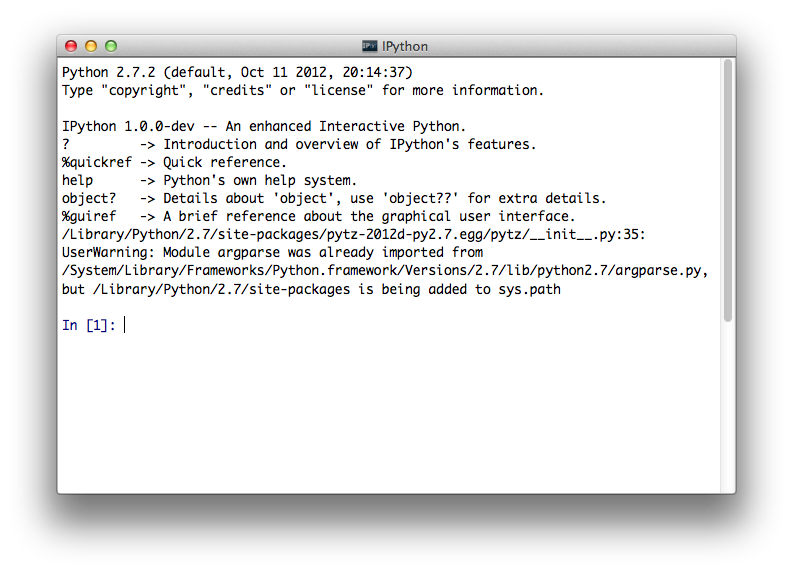
\includegraphics{files/images/qtconsole.png}
\caption{qtconsole}
\end{figure}\subsection{iPython Notebook}

IPython includes the \textbf{HTML notebook} featured here, as well as
support for \textbf{interactive data visualization} and easy
high-performance \textbf{parallel computing}.

    % Make sure that atleast 4 lines are below the HR
    \needspace{4\baselineskip}

    
        \vspace{6pt}
        \makebox[0.1\linewidth]{\smaller\hfill\tt\color{nbframe-in-prompt}In\hspace{4pt}{[}{]}:\hspace{4pt}}\\*
        \vspace{-2.65\baselineskip}
        \begin{ColorVerbatim}
            \vspace{-0.7\baselineskip}
            \begin{Verbatim}[commandchars=\\\{\}]
\PY{k}{def} \PY{n+nf}{f}\PY{p}{(}\PY{n}{x}\PY{p}{)}\PY{p}{:}
    \PY{k}{return} \PY{p}{(}\PY{n}{x}\PY{o}{-}\PY{l+m+mi}{3}\PY{p}{)}\PY{o}{*}\PY{p}{(}\PY{n}{x}\PY{o}{-}\PY{l+m+mi}{5}\PY{p}{)}\PY{o}{*}\PY{p}{(}\PY{n}{x}\PY{o}{-}\PY{l+m+mi}{7}\PY{p}{)}\PY{o}{+}\PY{l+m+mi}{85}

\PY{k+kn}{import} \PY{n+nn}{numpy} \PY{k+kn}{as} \PY{n+nn}{np}
\PY{n}{x} \PY{o}{=} \PY{n}{np}\PY{o}{.}\PY{n}{linspace}\PY{p}{(}\PY{l+m+mi}{0}\PY{p}{,} \PY{l+m+mi}{10}\PY{p}{,} \PY{l+m+mi}{200}\PY{p}{)}
\PY{n}{y} \PY{o}{=} \PY{n}{f}\PY{p}{(}\PY{n}{x}\PY{p}{)}
\PY{n}{plot}\PY{p}{(}\PY{n}{x}\PY{p}{,}\PY{n}{y}\PY{p}{)}
\end{Verbatim}

            
                \vspace{-0.2\baselineskip}
            
        \end{ColorVerbatim}
    
The notebook lets you document your workflow using either HTML or
Markdown.

The IPython Notebook consists of two related components:

\begin{itemize}
\item
  A JSON based Notebook document format for recording and distributing
  Python code and rich text.
\item
  A web-based user interface for authoring and running notebook
  documents.
\end{itemize}

The Notebook can be used by starting the Notebook server with the
command:

\begin{verbatim}
$ ipython notebook
\end{verbatim}

This initiates an \textbf{iPython engine}, which is a Python instance
that takes Python commands over a network connection. If we want to
enable inline plotting of figures via Matplotlib, we can add a
\texttt{-{}-pylab inline} flag to the command.

The \textbf{IPython controller} provides an interface for working with a
set of engines, to which one or more \textbf{iPython clients} can
connect.

The Notebook gives you everything that a browser gives you. For example,
you can embed images, videos, or entire websites.

    % Make sure that atleast 4 lines are below the HR
    \needspace{4\baselineskip}

    
        \vspace{6pt}
        \makebox[0.1\linewidth]{\smaller\hfill\tt\color{nbframe-in-prompt}In\hspace{4pt}{[}{]}:\hspace{4pt}}\\*
        \vspace{-2.65\baselineskip}
        \begin{ColorVerbatim}
            \vspace{-0.7\baselineskip}
            \begin{Verbatim}[commandchars=\\\{\}]
\PY{k+kn}{from} \PY{n+nn}{IPython.display} \PY{k+kn}{import} \PY{n}{HTML}
\PY{n}{HTML}\PY{p}{(}\PY{l+s}{"}\PY{l+s}{\PYZlt{}iframe src=http://fonnesbeck.github.io/Bios366 width=700 height=350\PYZgt{}\PYZlt{}/iframe\PYZgt{}}\PY{l+s}{"}\PY{p}{)}
\end{Verbatim}

            
                \vspace{-0.2\baselineskip}
            
        \end{ColorVerbatim}
    


    % Make sure that atleast 4 lines are below the HR
    \needspace{4\baselineskip}

    
        \vspace{6pt}
        \makebox[0.1\linewidth]{\smaller\hfill\tt\color{nbframe-in-prompt}In\hspace{4pt}{[}{]}:\hspace{4pt}}\\*
        \vspace{-2.65\baselineskip}
        \begin{ColorVerbatim}
            \vspace{-0.7\baselineskip}
            \begin{Verbatim}[commandchars=\\\{\}]
\PY{k+kn}{from} \PY{n+nn}{IPython.display} \PY{k+kn}{import} \PY{n}{YouTubeVideo}
\PY{n}{YouTubeVideo}\PY{p}{(}\PY{l+s}{"}\PY{l+s}{BS4Wd5rwNwE}\PY{l+s}{"}\PY{p}{)}
\end{Verbatim}

            
                \vspace{-0.2\baselineskip}
            
        \end{ColorVerbatim}
    
\subsubsection{Remote Code}

Use \texttt{\%load} to add remote code\subsubsection{Mathjax Support}

Mathjax ia a javascript implementation of LaTeX that allows equations to
be embedded into HTML. For example, this markup:

\begin{verbatim}
"""$$ \int_{a}^{b} f(x)\, dx \approx \frac{1}{2} \sum_{k=1}^{N} \left( x_{k} - x_{k-1} \right) \left( f(x_{k}) + f(x_{k-1}) \right). $$"""
\end{verbatim}

becomes this:

\[
\int_{a}^{b} f(x)\, dx \approx \frac{1}{2} \sum_{k=1}^{N} \left( x_{k} - x_{k-1} \right) \left( f(x_{k}) + f(x_{k-1}) \right).
\]\subsection{SymPy Support}

SymPy is a Python library for symbolic mathematics. It supports:

\begin{itemize}
\item
  polynomials
\item
  calculus
\item
  solving equations
\item
  discrete math
\item
  matrices
\end{itemize}

    % Make sure that atleast 4 lines are below the HR
    \needspace{4\baselineskip}

    
        \vspace{6pt}
        \makebox[0.1\linewidth]{\smaller\hfill\tt\color{nbframe-in-prompt}In\hspace{4pt}{[}{]}:\hspace{4pt}}\\*
        \vspace{-2.65\baselineskip}
        \begin{ColorVerbatim}
            \vspace{-0.7\baselineskip}
            \begin{Verbatim}[commandchars=\\\{\}]
\PY{k+kn}{from} \PY{n+nn}{sympy} \PY{k+kn}{import} \PY{o}{*}
\PY{o}{\PYZpc{}}\PY{k}{load\PYZus{}ext} \PY{n}{sympyprinting}
\PY{n}{x}\PY{p}{,} \PY{n}{y} \PY{o}{=} \PY{n}{symbols}\PY{p}{(}\PY{l+s}{"}\PY{l+s}{x y}\PY{l+s}{"}\PY{p}{)}
\end{Verbatim}

            
                \vspace{-0.2\baselineskip}
            
        \end{ColorVerbatim}
    


    % Make sure that atleast 4 lines are below the HR
    \needspace{4\baselineskip}

    
        \vspace{6pt}
        \makebox[0.1\linewidth]{\smaller\hfill\tt\color{nbframe-in-prompt}In\hspace{4pt}{[}{]}:\hspace{4pt}}\\*
        \vspace{-2.65\baselineskip}
        \begin{ColorVerbatim}
            \vspace{-0.7\baselineskip}
            \begin{Verbatim}[commandchars=\\\{\}]
\PY{n}{eq} \PY{o}{=} \PY{p}{(}\PY{p}{(}\PY{n}{x}\PY{o}{+}\PY{n}{y}\PY{p}{)}\PY{o}{*}\PY{o}{*}\PY{l+m+mi}{2} \PY{o}{*} \PY{p}{(}\PY{n}{x}\PY{o}{+}\PY{l+m+mi}{1}\PY{p}{)}\PY{p}{)}
\PY{n}{eq}
\end{Verbatim}

            
                \vspace{-0.2\baselineskip}
            
        \end{ColorVerbatim}
    


    % Make sure that atleast 4 lines are below the HR
    \needspace{4\baselineskip}

    
        \vspace{6pt}
        \makebox[0.1\linewidth]{\smaller\hfill\tt\color{nbframe-in-prompt}In\hspace{4pt}{[}{]}:\hspace{4pt}}\\*
        \vspace{-2.65\baselineskip}
        \begin{ColorVerbatim}
            \vspace{-0.7\baselineskip}
            \begin{Verbatim}[commandchars=\\\{\}]
\PY{n}{expand}\PY{p}{(}\PY{n}{eq}\PY{p}{)}
\end{Verbatim}

            
                \vspace{-0.2\baselineskip}
            
        \end{ColorVerbatim}
    


    % Make sure that atleast 4 lines are below the HR
    \needspace{4\baselineskip}

    
        \vspace{6pt}
        \makebox[0.1\linewidth]{\smaller\hfill\tt\color{nbframe-in-prompt}In\hspace{4pt}{[}{]}:\hspace{4pt}}\\*
        \vspace{-2.65\baselineskip}
        \begin{ColorVerbatim}
            \vspace{-0.7\baselineskip}
            \begin{Verbatim}[commandchars=\\\{\}]
\PY{p}{(}\PY{l+m+mi}{1}\PY{o}{/}\PY{n}{cos}\PY{p}{(}\PY{n}{x}\PY{p}{)}\PY{p}{)}\PY{o}{.}\PY{n}{series}\PY{p}{(}\PY{n}{x}\PY{p}{,} \PY{l+m+mi}{0}\PY{p}{,} \PY{l+m+mi}{6}\PY{p}{)}
\end{Verbatim}

            
                \vspace{-0.2\baselineskip}
            
        \end{ColorVerbatim}
    
\subsubsection{Magic functions}

IPython has a set of predefined `magic functions' that you can call with
a command line style syntax. These include:

\begin{itemize}
\item
  \texttt{\%run}
\item
  \texttt{\%edit}
\item
  \texttt{\%debug}
\item
  \texttt{\%timeit}
\item
  \texttt{\%paste}
\item
  \texttt{\%load\_ext}
\end{itemize}

    % Make sure that atleast 4 lines are below the HR
    \needspace{4\baselineskip}

    
        \vspace{6pt}
        \makebox[0.1\linewidth]{\smaller\hfill\tt\color{nbframe-in-prompt}In\hspace{4pt}{[}{]}:\hspace{4pt}}\\*
        \vspace{-2.65\baselineskip}
        \begin{ColorVerbatim}
            \vspace{-0.7\baselineskip}
            \begin{Verbatim}[commandchars=\\\{\}]
\PY{o}{\PYZpc{}}\PY{k}{lsmagic}
\end{Verbatim}

            
                \vspace{-0.2\baselineskip}
            
        \end{ColorVerbatim}
    
Timing the execution of code; the \texttt{timeit} magic exists both in
line and cell form:

    % Make sure that atleast 4 lines are below the HR
    \needspace{4\baselineskip}

    
        \vspace{6pt}
        \makebox[0.1\linewidth]{\smaller\hfill\tt\color{nbframe-in-prompt}In\hspace{4pt}{[}{]}:\hspace{4pt}}\\*
        \vspace{-2.65\baselineskip}
        \begin{ColorVerbatim}
            \vspace{-0.7\baselineskip}
            \begin{Verbatim}[commandchars=\\\{\}]
\PY{o}{\PYZpc{}}\PY{k}{timeit} \PY{n}{np}\PY{o}{.}\PY{n}{linalg}\PY{o}{.}\PY{n}{eigvals}\PY{p}{(}\PY{n}{np}\PY{o}{.}\PY{n}{random}\PY{o}{.}\PY{n}{rand}\PY{p}{(}\PY{l+m+mi}{100}\PY{p}{,}\PY{l+m+mi}{100}\PY{p}{)}\PY{p}{)}
\end{Verbatim}

            
                \vspace{-0.2\baselineskip}
            
        \end{ColorVerbatim}
    


    % Make sure that atleast 4 lines are below the HR
    \needspace{4\baselineskip}

    
        \vspace{6pt}
        \makebox[0.1\linewidth]{\smaller\hfill\tt\color{nbframe-in-prompt}In\hspace{4pt}{[}{]}:\hspace{4pt}}\\*
        \vspace{-2.65\baselineskip}
        \begin{ColorVerbatim}
            \vspace{-0.7\baselineskip}
            \begin{Verbatim}[commandchars=\\\{\}]
\PY{o}{\PYZpc{}\PYZpc{}}\PY{k}{timeit} \PY{n}{a} \PY{o}{=} \PY{n}{np}\PY{o}{.}\PY{n}{random}\PY{o}{.}\PY{n}{rand}\PY{p}{(}\PY{l+m+mi}{100}\PY{p}{,} \PY{l+m+mi}{100}\PY{p}{)}
\PY{n}{np}\PY{o}{.}\PY{n}{linalg}\PY{o}{.}\PY{n}{eigvals}\PY{p}{(}\PY{n}{a}\PY{p}{)}
\end{Verbatim}

            
                \vspace{-0.2\baselineskip}
            
        \end{ColorVerbatim}
    
IPython also creates aliases for a few common interpreters, such as
bash, ruby, perl, etc.

These are all equivalent to
\texttt{\%\%script \textless{}name\textgreater{}}

    % Make sure that atleast 4 lines are below the HR
    \needspace{4\baselineskip}

    
        \vspace{6pt}
        \makebox[0.1\linewidth]{\smaller\hfill\tt\color{nbframe-in-prompt}In\hspace{4pt}{[}{]}:\hspace{4pt}}\\*
        \vspace{-2.65\baselineskip}
        \begin{ColorVerbatim}
            \vspace{-0.7\baselineskip}
            \begin{Verbatim}[commandchars=\\\{\}]
\PY{o}{\PYZpc{}\PYZpc{}}\PY{k}{ruby}
\PY{n}{puts} \PY{l+s}{"}\PY{l+s}{Hello from Ruby \PYZsh{}\PYZob{}RUBY\PYZus{}VERSION\PYZcb{}}\PY{l+s}{"}
\end{Verbatim}

            
                \vspace{-0.2\baselineskip}
            
        \end{ColorVerbatim}
    


    % Make sure that atleast 4 lines are below the HR
    \needspace{4\baselineskip}

    
        \vspace{6pt}
        \makebox[0.1\linewidth]{\smaller\hfill\tt\color{nbframe-in-prompt}In\hspace{4pt}{[}{]}:\hspace{4pt}}\\*
        \vspace{-2.65\baselineskip}
        \begin{ColorVerbatim}
            \vspace{-0.7\baselineskip}
            \begin{Verbatim}[commandchars=\\\{\}]
\PY{o}{\PYZpc{}\PYZpc{}}\PY{k}{bash}
\PY{n}{echo} \PY{l+s}{"}\PY{l+s}{hello from \PYZdl{}BASH}\PY{l+s}{"}
\end{Verbatim}

            
                \vspace{-0.2\baselineskip}
            
        \end{ColorVerbatim}
    
IPython has an \texttt{rmagic} extension that contains a some magic
functions for working with R via rpy2. This extension can be loaded
using the \texttt{\%load\_ext} magic as follows:

    % Make sure that atleast 4 lines are below the HR
    \needspace{4\baselineskip}

    
        \vspace{6pt}
        \makebox[0.1\linewidth]{\smaller\hfill\tt\color{nbframe-in-prompt}In\hspace{4pt}{[}{]}:\hspace{4pt}}\\*
        \vspace{-2.65\baselineskip}
        \begin{ColorVerbatim}
            \vspace{-0.7\baselineskip}
            \begin{Verbatim}[commandchars=\\\{\}]
\PY{o}{\PYZpc{}}\PY{k}{load\PYZus{}ext} \PY{n}{rmagic}
\end{Verbatim}

            
                \vspace{-0.2\baselineskip}
            
        \end{ColorVerbatim}
    


    % Make sure that atleast 4 lines are below the HR
    \needspace{4\baselineskip}

    
        \vspace{6pt}
        \makebox[0.1\linewidth]{\smaller\hfill\tt\color{nbframe-in-prompt}In\hspace{4pt}{[}{]}:\hspace{4pt}}\\*
        \vspace{-2.65\baselineskip}
        \begin{ColorVerbatim}
            \vspace{-0.7\baselineskip}
            \begin{Verbatim}[commandchars=\\\{\}]
\PY{n}{x}\PY{p}{,}\PY{n}{y} \PY{o}{=} \PY{n}{arange}\PY{p}{(}\PY{l+m+mi}{10}\PY{p}{)}\PY{p}{,} \PY{n}{random}\PY{o}{.}\PY{n}{normal}\PY{p}{(}\PY{n}{size}\PY{o}{=}\PY{l+m+mi}{10}\PY{p}{)}
\end{Verbatim}

            
                \vspace{-0.2\baselineskip}
            
        \end{ColorVerbatim}
    


    % Make sure that atleast 4 lines are below the HR
    \needspace{4\baselineskip}

    
        \vspace{6pt}
        \makebox[0.1\linewidth]{\smaller\hfill\tt\color{nbframe-in-prompt}In\hspace{4pt}{[}{]}:\hspace{4pt}}\\*
        \vspace{-2.65\baselineskip}
        \begin{ColorVerbatim}
            \vspace{-0.7\baselineskip}
            \begin{Verbatim}[commandchars=\\\{\}]
\PY{o}{\PYZpc{}\PYZpc{}}\PY{k}{R} \PY{o}{-}\PY{n}{i} \PY{n}{x}\PY{p}{,}\PY{n}{y} \PY{o}{-}\PY{n}{o} \PY{n}{XYcoef}
\PY{n}{lm}\PY{o}{.}\PY{n}{fit} \PY{o}{\PYZlt{}}\PY{o}{-} \PY{n}{lm}\PY{p}{(}\PY{n}{y}\PY{o}{\PYZti{}}\PY{n}{x}\PY{p}{)}
\PY{n}{par}\PY{p}{(}\PY{n}{mfrow}\PY{o}{=}\PY{n}{c}\PY{p}{(}\PY{l+m+mi}{2}\PY{p}{,}\PY{l+m+mi}{2}\PY{p}{)}\PY{p}{)}
\PY{k}{print}\PY{p}{(}\PY{n}{summary}\PY{p}{(}\PY{n}{lm}\PY{o}{.}\PY{n}{fit}\PY{p}{)}\PY{p}{)}
\PY{n}{plot}\PY{p}{(}\PY{n}{lm}\PY{o}{.}\PY{n}{fit}\PY{p}{)}
\PY{n}{XYcoef} \PY{o}{\PYZlt{}}\PY{o}{-} \PY{n}{coef}\PY{p}{(}\PY{n}{lm}\PY{o}{.}\PY{n}{fit}\PY{p}{)}
\end{Verbatim}

            
                \vspace{-0.2\baselineskip}
            
        \end{ColorVerbatim}
    


    % Make sure that atleast 4 lines are below the HR
    \needspace{4\baselineskip}

    
        \vspace{6pt}
        \makebox[0.1\linewidth]{\smaller\hfill\tt\color{nbframe-in-prompt}In\hspace{4pt}{[}{]}:\hspace{4pt}}\\*
        \vspace{-2.65\baselineskip}
        \begin{ColorVerbatim}
            \vspace{-0.7\baselineskip}
            \begin{Verbatim}[commandchars=\\\{\}]
\PY{n}{XYcoef}
\end{Verbatim}

            
                \vspace{-0.2\baselineskip}
            
        \end{ColorVerbatim}
    
\subsection{Exporting and Converting Notebooks}

In IPython 1.0, one can convert an \texttt{.ipynb} notebook document
file into various static formats via the \texttt{nbconvert} tool.
Currently, nbconvert is a command line tool, run as a script using
IPython.

    % Make sure that atleast 4 lines are below the HR
    \needspace{4\baselineskip}

    
        \vspace{6pt}
        \makebox[0.1\linewidth]{\smaller\hfill\tt\color{nbframe-in-prompt}In\hspace{4pt}{[}{]}:\hspace{4pt}}\\*
        \vspace{-2.65\baselineskip}
        \begin{ColorVerbatim}
            \vspace{-0.7\baselineskip}
            \begin{Verbatim}[commandchars=\\\{\}]
\PY{o}{!}ipython nbconvert --to latex Section2\PYZus{}1-IPython.ipynb
\end{Verbatim}

            
                \vspace{-0.2\baselineskip}
            
        \end{ColorVerbatim}
    


    % Make sure that atleast 4 lines are below the HR
    \needspace{4\baselineskip}

    
        \vspace{6pt}
        \makebox[0.1\linewidth]{\smaller\hfill\tt\color{nbframe-in-prompt}In\hspace{4pt}{[}{]}:\hspace{4pt}}\\*
        \vspace{-2.65\baselineskip}
        \begin{ColorVerbatim}
            \vspace{-0.7\baselineskip}
            \begin{Verbatim}[commandchars=\\\{\}]
\PY{o}{\PYZpc{}}\PY{k}{load} \PY{n}{Section2\PYZus{}1}\PY{o}{-}\PY{n}{IPython}\PY{o}{.}\PY{n}{tex}
\end{Verbatim}

            
                \vspace{-0.2\baselineskip}
            
        \end{ColorVerbatim}
    
Currently, \texttt{nbconvert} supports HTML (default), LaTeX, Mardown,
reStructuredText, Python and HTML5 slides for presentations.A very useful online service is the
\href{http://nbviewer.ipython.org}{IPython Notebook Viewer} which allows
you to display your notebook as a static HTML page, which is useful for
sharing with others:

    % Make sure that atleast 4 lines are below the HR
    \needspace{4\baselineskip}

    
        \vspace{6pt}
        \makebox[0.1\linewidth]{\smaller\hfill\tt\color{nbframe-in-prompt}In\hspace{4pt}{[}{]}:\hspace{4pt}}\\*
        \vspace{-2.65\baselineskip}
        \begin{ColorVerbatim}
            \vspace{-0.7\baselineskip}
            \begin{Verbatim}[commandchars=\\\{\}]
\PY{k+kn}{from} \PY{n+nn}{IPython.display} \PY{k+kn}{import} \PY{n}{HTML}
\PY{n}{HTML}\PY{p}{(}\PY{l+s}{"}\PY{l+s}{\PYZlt{}iframe src=http://nbviewer.ipython.org/4042018 width=700 height=350\PYZgt{}\PYZlt{}/iframe\PYZgt{}}\PY{l+s}{"}\PY{p}{)}
\end{Verbatim}

            
                \vspace{-0.2\baselineskip}
            
        \end{ColorVerbatim}
    
\subsection{Reproducible Research}

\begin{quote}
reproducing conclusions from a single experiment based on the
measurements from that experiment
\end{quote}

The most basic form of reproducibility is a complete description of the
data and associated analyses (including code!) so the results can be
\emph{exactly} reproduced by others.

Reproducing calculations can be onerous, even with one's own work!

Scientific data are becoming larger and more complex, making simple
descriptions inadequate for reproducibility. As a result, most modern
research is irreproducible without tremendous effort.

\emph{*} Reproducible research is not yet part of the culture of science
in general, or scientific computing in particular. \emph{*}\subsection{Scientific Computing Workflow}

There are a number of steps to scientific endeavors that involve
computing:

\begin{figure}[htbp]
\centering
\includegraphics{http://f.cl.ly/items/3B0l063n2T0H1p041U3L/workflow.png}
\caption{workflow}
\end{figure}

Many of the standard tools impose barriers between one or more of these
steps. This can make it difficult to iterate, reproduce work.

The IPython notebook eliminates or reduces these barriers to
reproducibility.\section{Parallel iPython}Before running the next cell, make sure you have first started your
cluster, you can use the \href{/\#tab2}{clusters tab in the dashboard}
to do so.

    % Make sure that atleast 4 lines are below the HR
    \needspace{4\baselineskip}

    
        \vspace{6pt}
        \makebox[0.1\linewidth]{\smaller\hfill\tt\color{nbframe-in-prompt}In\hspace{4pt}{[}{]}:\hspace{4pt}}\\*
        \vspace{-2.65\baselineskip}
        \begin{ColorVerbatim}
            \vspace{-0.7\baselineskip}
            \begin{Verbatim}[commandchars=\\\{\}]
\PY{k+kn}{from} \PY{n+nn}{IPython.parallel} \PY{k+kn}{import} \PY{n}{Client}
\PY{n}{client} \PY{o}{=} \PY{n}{Client}\PY{p}{(}\PY{p}{)}
\PY{n}{dv} \PY{o}{=} \PY{n}{client}\PY{o}{.}\PY{n}{direct\PYZus{}view}\PY{p}{(}\PY{p}{)}
\end{Verbatim}

            
                \vspace{-0.2\baselineskip}
            
        \end{ColorVerbatim}
    


    % Make sure that atleast 4 lines are below the HR
    \needspace{4\baselineskip}

    
        \vspace{6pt}
        \makebox[0.1\linewidth]{\smaller\hfill\tt\color{nbframe-in-prompt}In\hspace{4pt}{[}{]}:\hspace{4pt}}\\*
        \vspace{-2.65\baselineskip}
        \begin{ColorVerbatim}
            \vspace{-0.7\baselineskip}
            \begin{Verbatim}[commandchars=\\\{\}]
\PY{n+nb}{len}\PY{p}{(}\PY{n}{dv}\PY{p}{)}
\end{Verbatim}

            
                \vspace{-0.2\baselineskip}
            
        \end{ColorVerbatim}
    


    % Make sure that atleast 4 lines are below the HR
    \needspace{4\baselineskip}

    
        \vspace{6pt}
        \makebox[0.1\linewidth]{\smaller\hfill\tt\color{nbframe-in-prompt}In\hspace{4pt}{[}{]}:\hspace{4pt}}\\*
        \vspace{-2.65\baselineskip}
        \begin{ColorVerbatim}
            \vspace{-0.7\baselineskip}
            \begin{Verbatim}[commandchars=\\\{\}]
\PY{k}{def} \PY{n+nf}{where\PYZus{}am\PYZus{}i}\PY{p}{(}\PY{p}{)}\PY{p}{:}
    \PY{k+kn}{import} \PY{n+nn}{os}
    \PY{k+kn}{import} \PY{n+nn}{socket}
    
    \PY{k}{return} \PY{l+s}{"}\PY{l+s}{In process with pid \PYZob{}0\PYZcb{} on host: }\PY{l+s}{'}\PY{l+s}{\PYZob{}1\PYZcb{}}\PY{l+s}{'}\PY{l+s}{"}\PY{o}{.}\PY{n}{format}\PY{p}{(}
        \PY{n}{os}\PY{o}{.}\PY{n}{getpid}\PY{p}{(}\PY{p}{)}\PY{p}{,} \PY{n}{socket}\PY{o}{.}\PY{n}{gethostname}\PY{p}{(}\PY{p}{)}\PY{p}{)}
\end{Verbatim}

            
                \vspace{-0.2\baselineskip}
            
        \end{ColorVerbatim}
    


    % Make sure that atleast 4 lines are below the HR
    \needspace{4\baselineskip}

    
        \vspace{6pt}
        \makebox[0.1\linewidth]{\smaller\hfill\tt\color{nbframe-in-prompt}In\hspace{4pt}{[}{]}:\hspace{4pt}}\\*
        \vspace{-2.65\baselineskip}
        \begin{ColorVerbatim}
            \vspace{-0.7\baselineskip}
            \begin{Verbatim}[commandchars=\\\{\}]
\PY{n}{where\PYZus{}am\PYZus{}i\PYZus{}direct\PYZus{}results} \PY{o}{=} \PY{n}{dv}\PY{o}{.}\PY{n}{apply}\PY{p}{(}\PY{n}{where\PYZus{}am\PYZus{}i}\PY{p}{)}
\PY{n}{where\PYZus{}am\PYZus{}i\PYZus{}direct\PYZus{}results}\PY{o}{.}\PY{n}{get}\PY{p}{(}\PY{p}{)}
\end{Verbatim}

            
                \vspace{-0.2\baselineskip}
            
        \end{ColorVerbatim}
    
\subsection{Links and References}\href{http://nbviewer.ipython.org}{IPython Notebook Viewer} Displays
static HTML versions of notebooks, and includes a gallery of notebook
examples.\href{https://notebookcloud.appspot.com}{NotebookCloud} A service that
allows you to launch and control IPython Notebook servers on Amazon EC2
from your browser.\href{http://ged.msu.edu/papers/2012-diginorm/}{A Reference-Free
Algorithm for Computational Normalization of Shotgun Sequencing Data} A
landmark example of reproducible research in genomics: Git repo, iPython
notebook, data and scripts.\begin{center}\rule{3in}{0.4pt}\end{center}

    % Make sure that atleast 4 lines are below the HR
    \needspace{4\baselineskip}

    
        \vspace{6pt}
        \makebox[0.1\linewidth]{\smaller\hfill\tt\color{nbframe-in-prompt}In\hspace{4pt}{[}54{]}:\hspace{4pt}}\\*
        \vspace{-2.65\baselineskip}
        \begin{ColorVerbatim}
            \vspace{-0.7\baselineskip}
            \begin{Verbatim}[commandchars=\\\{\}]
\PY{k+kn}{from} \PY{n+nn}{IPython.core.display} \PY{k+kn}{import} \PY{n}{HTML}
\PY{k}{def} \PY{n+nf}{css\PYZus{}styling}\PY{p}{(}\PY{p}{)}\PY{p}{:}
    \PY{n}{styles} \PY{o}{=} \PY{n+nb}{open}\PY{p}{(}\PY{l+s}{"}\PY{l+s}{styles/custom.css}\PY{l+s}{"}\PY{p}{,} \PY{l+s}{"}\PY{l+s}{r}\PY{l+s}{"}\PY{p}{)}\PY{o}{.}\PY{n}{read}\PY{p}{(}\PY{p}{)}
    \PY{k}{return} \PY{n}{HTML}\PY{p}{(}\PY{n}{styles}\PY{p}{)}
\PY{n}{css\PYZus{}styling}\PY{p}{(}\PY{p}{)}
\end{Verbatim}

            
                \vspace{-0.2\baselineskip}
            
        \end{ColorVerbatim}
    

    

        % If the first block is an image, minipage the image.  Else
        % request a certain amount of space for the input text.
        \needspace{4\baselineskip}
        
        

            % Add document contents.
            
                \makebox[0.1\linewidth]{\smaller\hfill\tt\color{nbframe-out-prompt}Out\hspace{4pt}{[}54{]}:\hspace{4pt}}\\*
                \vspace{-2.55\baselineskip}\begin{InvisibleVerbatim}
                \vspace{-0.5\baselineskip}
\begin{alltt}<IPython.core.display.HTML object at 0x1162617d0>\end{alltt}

            \end{InvisibleVerbatim}
            
        
    

        

        \renewcommand{\indexname}{Index}
        \printindex

    % End of document
    \end{document}


